\documentclass[12pt]{article}
\usepackage[utf8]{inputenc}
\usepackage[spanish]{babel}
%\usepackage{graphicx}
\usepackage{url}
\usepackage{listings}

\usepackage{tikz}
\usepackage{graphicx}
\usepackage{lscape}
\usepackage{amsmath}
\usepackage{textcomp}
\usepackage{geometry}
\usetikzlibrary{babel}
\usetikzlibrary{shadows}
\usetikzlibrary{arrows} 
\usetikzlibrary{decorations.markings}
\usetikzlibrary{matrix,positioning,calc}
\usetikzlibrary{decorations.pathmorphing}
\tikzset{
    %Define standard arrow tip
    >=stealth',
    %Define style for boxes
    punkt/.style={
           rectangle,
           rounded corners,
           draw=black, very thick,
           text width=6.5em,
           minimum height=2em,
           text centered},
    % Define arrow style
    pil/.style={
           ->,
           thick,
           shorten <=2pt,
           shorten >=2pt,}
}
\tikzset{%
  block/.style    = {draw, thick, rectangle},
  sum/.style      = {draw, circle, node distance = 2cm}, % Adder
  input/.style    = {coordinate}, % Input
  output/.style   = {coordinate} % Output
}

\newcommand*\keystroke[1]{%
  \tikz[baseline=(key.base)]
    \node[%
      draw,
      fill=white,
      drop shadow={shadow xshift=0.25ex,shadow yshift=-0.25ex,fill=black,opacity=0.75},
      rectangle,
      minimum width=0.6cm,
      minimum height=0.5cm,
      rounded corners=2pt,
      inner sep=1pt,
      line width=0.5pt,
      font=\scriptsize\sffamily
    ](key) {#1\strut}
  ;
}
\begin{document}

\begin{titlepage}
\begin{tikzpicture}[remember picture,overlay]
% draw image
\node[inner sep=0,opacity=0.4] at (current page.center)
{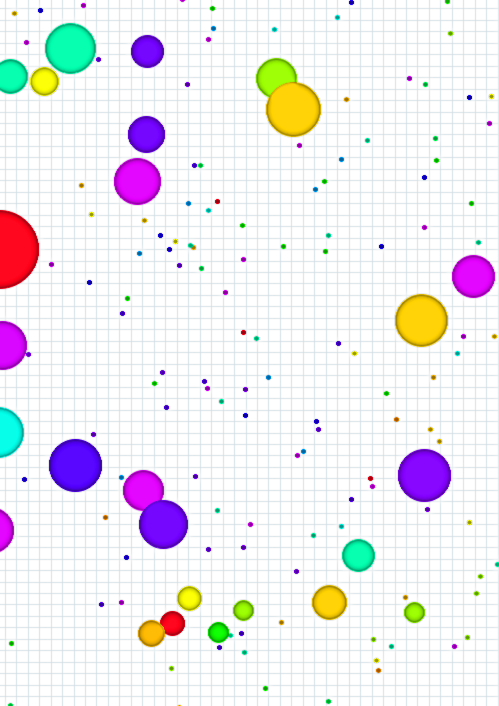
\includegraphics[width=\paperwidth,height=\paperheight]{caratula.png}};
\end{tikzpicture}

\newcommand{\HRule}{\rule{\linewidth}{0.5mm}} % Defines a new command for the horizontal lines, change thickness here

\center % Center everything on the page
 
%----------------------------------------------------------------------------------------
%   HEADING SECTIONS
%----------------------------------------------------------------------------------------

\textsc{\LARGE Universidad Nacional de Rosario}\\[0.5cm] % Name of your university/college
\textsc{\Large Ciencias de la Computación}\\[1.5cm] % Major heading such as course name
\textsc{\Large Análisis de Lenguajes de Programación}\\[0.5cm] % Major heading such as course name
\textsc{\large Trabajo Final}\\[0.5cm] % Minor heading such as course title


%----------------------------------------------------------------------------------------
%   TITLE SECTION
%----------------------------------------------------------------------------------------

\HRule \\[0.4cm]
{ \huge \bfseries AGARSIMU}\\[0.4cm] % Title of your document
\HRule \\[1cm]
 
%----------------------------------------------------------------------------------------
%   AUTHOR SECTION
%----------------------------------------------------------------------------------------

%\begin{minipage}{0.4\textwidth}
%\begin{flushleft} \large
%\emph{Autor}\\
%\textsc{Martín Villagra} % Your name
%\end{flushleft}
%\end{minipage}

%\begin{minipage}{0.4\textwidth}
%\begin{flushright} \large
%\emph{Supervisor} \\
%Dr. James \textsc{Smith} % Supervisor's Name
%\end{flushright}
%\end{minipage}\\[2cm]

% If you don't want a supervisor, uncomment the two lines below and remove the section above
\Large \emph{Autor}\\
\textsc{Martín Villagra}\\[1cm] % Your name

%----------------------------------------------------------------------------------------
%   DATE SECTION
%----------------------------------------------------------------------------------------

{\large \today}\\[0.5cm] % Date, change the \today to a set date if you want to be precise

%----------------------------------------------------------------------------------------
%   LOGO SECTION
%----------------------------------------------------------------------------------------


\includegraphics[width=4cm]{logo-unr.png}\\[1cm] % Include a department/university logo - this will require the graphicx package
 
%----------------------------------------------------------------------------------------

\end{titlepage}

\section{Descripción}
AgarSimu es un simulador de una versión simplificada\footnote{Los jugadores no se pueden dividir o regalar masa.} del popular juego agar.io\footnote{\url{https://en.wikipedia.org/wiki/Agar.io}, \url{http://agar.io}}. Provee una interfaz para diseñar inteligencias artificiales\footnote{\url{https://en.wikipedia.org/wiki/Artificial_intelligence}} (o más específicamente bots\footnote{\url{https://en.wikipedia.org/wiki/Video_game_bot}}) que responden a su entorno y la evolución del mismo en el tiempo. A su vez permite ejecutar estos agentes en conjunto dentro de un mundo (instancia del juego).
\section{Instalación}
Pre-requitisito SDL library. Para Ubuntu:
\begin{lstlisting}[language=bash]
  $ apt-get install libsdl1.2-dev libsdl-gfx1.2-dev
\end{lstlisting}

Una vez instalada la SDL, descargar el simulador e ingresar en la carpeta del mismo:

\begin{lstlisting}[language=bash]
  $ git clone https://github.com/mvpossum/agarsimu
  $ cd agarsimu
\end{lstlisting}

El simulador se puede instalar usando cabal-install. Se puede instalarlo localmente (para el usuario actual):

\begin{lstlisting}[language=bash]
  $ cabal install
\end{lstlisting}

O bien en una sandbox: (recomendado)
\begin{lstlisting}[language=bash]
  $ cabal sanbox init
  $ cabal install
\end{lstlisting}

Puede ejecutar una prueba del paquete haciendo:
\begin{lstlisting}[language=bash]
  $ cabal test
\end{lstlisting}

Dependiendo de cuantos paquetes haya que bajar, esto suele tardar bastante, especialmente si se usa una sandbox.
\section{Tutorial de uso}
\subsection{Ejecutar la simulación}
El procedimiento es crear un builder y luego pasarselo a la función \emph{runSimulation}. Un builder crea el estado inicial de la simulación. Este estado contiene las bolas y las AI asociadas a cada cada una de las bolas.

A modo introductorio se muestra un uso simple del paquete en el archivo \mbox{\emph{test/HelloWorld.hs}}
\subsection{Controles de la simulación}
\begin{itemize}
\item Para cerrar la simulación presione \keystroke{q}.
\item Para hacer zoom utilice la rueda del mouse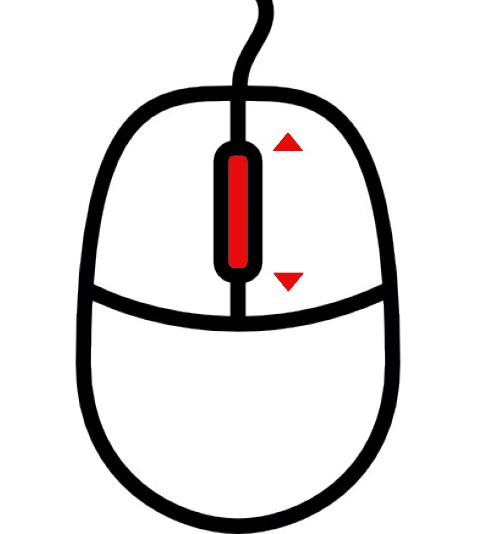
\includegraphics[width=0.8cm]{mouse-wheel.png}.
\item Para mover la cámara mantenga presionado el click izquierdo 
\includegraphics[width=0.8cm]{mouse-click.png} y mueva el mouse.
\item Para aumentar/disminuir la velocidad presione \keystroke{+}/\keystroke{-} del teclado númerico o bien \keystroke{w}/\keystroke{s}.
\end{itemize}
\subsection{Creación de AIs}
\begin{lstlisting}[language=haskell]
type Vector = (Double, Double)
type Environment = (Vector, Bola, [Bola])
\end{lstlisting}
Para nuestros fines, una AI es una función que recibe la información de su entorno y devuelve la dirección en la que moverse. Vamos a definir el entorno como una una tripleta (Vector, Bola, [Bola]) que representa respectivamente el tamaño del mapa, información referente a la bola que controla la AI e información de las otras bolas.
Si no nos interesa el factor tiempo en nuestro bot, podemos utilizar la función \emph{liftAI}:
\begin{lstlisting}[language=haskell]
liftAI :: (Environment -> Vector) -> AI
\end{lstlisting}
Si queremos tener una especie de memoria o estado, pero sin preocuparnos por el factor tiempo, se provee la función \emph{liftAISF}:
\begin{lstlisting}[language=haskell]
-- | Tenemos que aportar el estado inicial ahora
liftAISF :: m -> (Environment -> State m Vector) -> AI
\end{lstlisting}
Para los casos en los que si importe el tiempo, tenemos que recurrir a una definición más poderosa que se verá a continuación.
\subsubsection{Wires con Netwire}
Las AI son modeladas usando wires, el tipo provisto por la librería de FRP ``Netwire''. Se recomienda leer la bibliografía presentada al final para un mejor entendimiento. Un Wire, que es un tipo especial de Arrow autómata, viene dado por el tipo:
\begin{lstlisting}[language=haskell]
data Wire s e m a b
\end{lstlisting}
Un Wire representa una `función' reactiva\footnote{Cuyo comportamiento varía con el tiempo.}. Más específicamente, es una función que toma de argumentos:
\begin{itemize}
\item Un valor de tipo $s$ que contiene de alguna forma el tiempo transcurrido.
\item Una valor de tipo $a$.
\end{itemize}
De estos argumentos el Wire:
\begin{itemize}
\item O bien devuelve un valor de tipo $b$ o se `inhibe' con un valor de tipo $e$ (\textbf{e}rror).
\item Crea un nuevo Wire s e m a b.
\end{itemize}
Visto esto podemos pensar a un Wire como:
\begin{lstlisting}[language=haskell]
 newtype Wire s e m a b =
     Wire {
       stepWire :: s -> a -> m (Either e b, Wire s e m a b)
     }
\end{lstlisting}
Notar como al devolver una nueva instancia de sí mismo, el Wire puede variar su comportamiento a medida que pasa el tiempo. Si bien esta definición parece ser excesivamente complicada, efectivamente vuelve más intuitiva la semántica de los Wires.



En cuanto a la creación de Wires se debe tener a mano la referencia de Netwire\footnote{mencionada en la bibliografía}, puesto que esta provee numerosas funciones para crear y combinar Wires. Por nombrar algunas:
\begin{itemize}
\item $(a<|>b)$ se comporta siempre como $a$ a menos que el mismo se inhiba, en cuyo caso se comporta como $b$.
\item $(a-->b)$ se comporta como $a$ hasta que se inhiba por primera vez, luego pasa a comportarse siempre como $b$.
\end{itemize}


En nuestro caso la variable s es la que aconseja el paquete por defecto para llevar cuenta del tiempo, $e$ será el tipo $()$\footnote{La inhibición de la AI es equivalente a dejar de jugar, por lo que no conviene inhibirse en la mayoría de los casos.}. También se embebió la mónada Rand por sí por alguna razón se desea agregar algún comportamiento aleatorio al bot.

Con lo ya dicho podemos mostrar finalmente el tipo de las AI:
\begin{lstlisting}[language=haskell]
type Time = NominalDiffTime
type RandomWire = Wire (Timed Time ()) () (Rand StdGen)
type AI = RandomWire Environment Vector
\end{lstlisting}

\section{Esquema de la simulación}
La simulación se hizo aprovechando los Wires. En particular los mismos permiten estructurar el sistema en ``cajas negras'' que se pueden combinar para crear cajas más complejas.

El esquema presentado en el anexo muestra de forma simplificada la estructura de la simulación, el mismo sólo indica el flujo reactivo del sistema (los argumentos estáticos de las funciones no se muestran) por cada paso de la simulación. Cada caja representa un Wire.

\section{Organización del código}
El código del simulador se encuentra en la carpeta AgarSimu. Se explica a continuación el contenido de cada módulo.
\begin{itemize}
\item \textbf{Input.hs} Define los wires que procesan los eventos del usuario (mouse y teclado)
\item \textbf{Render.hs} Provee funciones para renderizar el juego en pantalla.
\item \textbf{Bola.hs} Contiene funciones que modelan el comportamiento de una bola en el juego. Es decir como varía su posición, velocidad, control de colisiones, etc.
\item \textbf{Core.hs} Combina los módulos listados arriba para ejecutar el juego.
\item \textbf{Scene.hs} Define un mini EDSL para crear las escenas (el estado inicial de la simulación).
\item \textbf{PublicEntities.hs} Define los tipos usados por el usuario final. Se separó del resto para proveer una interfaz más clara. 
\item \textbf{PreFab.hs} Se incluyen funciones útiles que podrían ser útiles para el desarollo de las AIs. 
\item \textbf{Utils.hs} Funciones de utilidad para los otros módulos. Aquí se definen, por ejemplo, funciones para combinar muchos wires en uno (wires de wires). 
\end{itemize}

\section{Detalles de implementación}
\subsection{Control de velocidad}
Como se puede apreciar en el diagrama, la velocidad controla el usuario afecta a la simulación tanto como al renderizado. Más específicamente cuando se aumenta la velocidad:
\begin{itemize}
\item Aumenta la velocidad de cada una de las bolas, dentro de la lógica del juego.
\item El aumento excesivo de velocidad conduce a errores de precisión dado que la simulación en realidad es un proceso discreto. Para disminuir este efecto, se implementa otra forma de aumentar la velocidad de simulación sin perder precisión. Consiste en no renderizar todos los pasos individuales que produce la simulación. 
\end{itemize} 
\subsection{Posición}
Un detalle interesente que permiten los Wires es expresar la posición de la bola como la integral de la velocidad, su implementación puede verse en \emph{Bola.hs}.
\subsection{combine y dynMulticast}
Para realizar \emph{aiswire} y \emph{foodGenerator} se tuvieron que crear funciones que toman un conjunto de wires y crean un wire que contiene el comportamiento de todos. Ver su implementación en \textbf{Utils.hs}, especialmente sus tipos, que son bastante intuitivos.

\section{Bibliografía}
\begin{itemize}
\item Introducción a FRP
\begin{itemize}
\item Lambda Jam 2015 - Conal Elliott - The Essence and Origins of Functional Reactive Programming,
\url{https://www.youtube.com/watch?v=j3Q32brCUAI}
\item Lambda Jam 2015 - Conal Elliott - A More Elegant Specification for FRP, \url{https://www.youtube.com/watch?v=teRC_Lf61Gw}
\end{itemize}
\item Arrows
\begin{itemize}
\item Haskell/Arrow tutorial, \url{https://en.wikibooks.org/wiki/Haskell/Arrow_tutorial}
\item How does ArrowLoop work? Also, mfix?, \url{http://stackoverflow.com/questions/6976944/how-does-arrowloop-work-also-mfix}
\item How does this definition of ArrowLoop.loop work?, \url{http://stackoverflow.com/questions/9856342/how-does-this-definition-of-arrowloop-loop-work}
\item GHC Language Features, Arrow notation, \url{https://downloads.haskell.org/~ghc/7.8.4/docs/html/users_guide/arrow-notation.html}
\end{itemize}
\item Wires
\begin{itemize}
\item Oliver Charles Blog, Getting Started with Netwire and SDL, \url{https://ocharles.org.uk/blog/posts/2013-08-01-getting-started-with-netwire-and-sdl.html}
\item Today in Code, Almost a Netwire 5 Tutorial, \url{http://todayincode.tumblr.com/post/96914679355/almost-a-netwire-5-tutorial}
\item Readme de Netwire, \url{http://hackage.haskell.org/package/netwire-5.0.1#readme}
\item Referencia de Netwire, \url{hackage.haskell.org/package/netwire-5.0.1}

\end{itemize}
\item Juegos de ejemplo
\begin{itemize}
\item Oliver Charles Blog, Asteroids \& Netwire, \url{
https://ocharles.org.uk/blog/posts/2013-08-18-asteroids-in-netwire.html}
\item Nathan Hüsken Blog, Breakout - Improved and with netwire, \url{http://jshaskell.blogspot.com.ar/2012/11/breakout-improved-and-with-netwire.html}
\end{itemize}
\end{itemize}

\newgeometry{left=2.5cm,right=1cm, bottom=3cm}
\begin{landscape}
\section*{Anexo: Esquema de la simulación}
\begin{tikzpicture}[auto, thick, node distance=2cm, >=triangle 45]
\draw
	node at (0, 0)[block] (readEvents) {readEvents}
	node [input, name=input1, right of=readEvents] {} 
	node [block, right of=input1](mouseCam) {
		\begin{tikzpicture}
		\draw node [] (mouseCam2) {mouseCam}
		      node [block, below =0cm of mouseCam2, text width=1.5cm](handler) {leftCick\\Handler};
		\end{tikzpicture}}
	node [block, above of =mouseCam](speedHandler) {speedHandler}
	node [block, below of =mouseCam](quitHandler) {quitHandler}
	node [input, name=input2, right of=mouseCam] {};
	\draw[->](readEvents) |- node[near end] {events}(speedHandler);
	\draw[->](readEvents) |- node[near end] {events}(quitHandler);
	\draw[->](readEvents) -- node{events}(mouseCam);

	\draw [thick](-1.5,-3) rectangle (6,3.5);
	\node at (-1.5,3) [above=5mm, right=0mm] {\textsc{inputLogic}}
	node [input, name=input2, right=1.5cm of mouseCam] {};


	\draw node[above right =4.5cm and 5cm of mouseCam] (aiswire) {\large aiswire};
	\draw node[block, below =0.5cm of aiswire, text width=2cm](b1) {\footnotesize bolaLogic \\ \begin{tikzpicture}
	\draw node[block, text width=0.5cm] {\scriptsize AI};
	\end{tikzpicture}};
	\draw node[block, below =0.2cm of b1, text width=2cm](b2) {\footnotesize bolaLogic \\ \begin{tikzpicture}
	\draw node[block, text width=0.5cm] {\scriptsize AI};
	\end{tikzpicture}};
	\draw node[block, below =0.2cm of b2, text width=2cm](b3) {\footnotesize bolaLogic \\ \begin{tikzpicture}
	\draw node[block, text width=0.5cm] {\scriptsize AI};
	\end{tikzpicture}};
	\draw node[below = 0.2cm of b3, text width=2cm]{$\vdots$};
	\draw node[right =1.2cm of b2] (suma1){\Large \textopenbullet};
	\draw node[circle,draw,right =1cm of suma1] (suma3){$++$};
	\draw node[left =1.7cm of b2] (input4){\Large \textopenbullet};
	\draw [thick](9.5,0) rectangle (12.5,6.2);
	\draw[->](b1) -- node[near end]{Bola}(13.5, 4.45) -| (suma1);
	\draw[->](b2) -- node{Bola}(suma1);
	\draw[->](b3) -| node[near end]{Bola}(suma1);
	\draw[->](input4) -- node{Env.}(b2);
	\draw[->](input4) |- node[near end]{Env.}(b3);
	\draw[->](input4) |- node[near end]{Env.}(b1);
	\draw[->](14.2, 3.15) |- node[near end]{[Bola]}(suma3);
	\draw[->](suma3) -- (15.65,4.15) -- (15.65, 7) -- node[above]{[Bola]}(10.5, 7) -- (7, 7) |- (input4);


	\draw node[below right =0.5cm and 4.0cm of mouseCam] (foodGenerator) {\large foodGenerator};
	\draw node[block, below =0.5cm of foodGenerator, text width=2cm](f1) {\footnotesize foodLogic};
	\draw node[block, below =0.2cm of f1, text width=2cm](f2) {\footnotesize foodLogic};
	\draw node[block, below =0.2cm of f2, text width=2cm](f3) {\footnotesize foodLogic};
	\draw node[below = 0.2cm of f3, text width=2cm]{$\vdots$};
	\draw node[right =2cm of f2] (suma2){\Large \textopenbullet};
	\draw [thick](9,-6.2) rectangle (12.7,-1);
	\draw[->](f1) -- node[near end]{Bola}(14, -2.95) -| (suma2);
	\draw[->](f2) -- node{Bola}(suma2);
	\draw[->](f3) -| node[near end]{Bola}(suma2);
	\draw[->] (14.8,-3.8) -| node[near end]{[Bola]}(suma3);
	\draw[->] (suma1) -- (14.3,2) -- (14.3,-0.5)--(7,-0.5) -- (7, -2) |- (f3);
	\draw[->] (suma1) -- (14.3,2) -- (14.3,-0.5)--(7,-0.5) -- (7, -2) |- (f2);
	\draw[->] (suma1) -- (14.3,2) -- (14.3,-0.5)--(7,-0.5) -- node[near end]{[Bola]}(7, -2) |- (f1);
	\draw[->] (speedHandler) -- node[below,near end]{speed}(input4);
	
	\draw [thick](6.5,-7) rectangle (17,8.5);
	\node at (6.5,8) [above=5mm, right=0mm] {\textsc{gameLogic}};
	
	\draw node[block, right=3cm of suma3] (renderLogic){\textsc{renderLogic}};
	\draw[->] (suma3) -- node[near end]{[Bola]}(renderLogic);
	\draw[->] (mouseCam) -- (6.3, 0) -- (6.3, -7.5)-| node[near end]{Camera}(renderLogic);
	\draw[->] (speedHandler) -- (6.3, 2) -- (6.3, 9)-| node[near end]{speed}(renderLogic);
\end{tikzpicture}
\end{landscape}
\restoregeometry
\end{document}